\documentclass[hyperref={pdfpagelabels=false}]{beamer}
\usepackage{lmodern}
\usepackage{multicol}
\usepackage{amsmath}
\usepackage{amssymb}
\usepackage{epsfig}
\usepackage{graphics}
\usepackage{epstopdf}
%\usepackage{mdframed}
\usepackage{xcolor}
\usepackage{color}
\usepackage{tikz}
\usepackage{array}
\usepackage[compatibility=false]{caption}
\usepackage{subcaption}

%\usepackage{booktabs}
%\usepackage{threeparttable}
%\usepackage{multirow}

\newcommand*\circled[1]{\tikz[baseline=(char.base)]{
            \node[shape=circle,draw,inner sep=2pt] (char) {#1};}}

\definecolor{amethyst}{rgb}{0.6, 0.4, 0.8}
\definecolor{brightube}{rgb}{0.82, 0.62, 0.91}
\definecolor{babyblue}{rgb}{0.54, 0.81, 0.94}
\definecolor{darkgreen}{rgb}{0.0, 0.5, 0.0}

\newtheorem{assumption}{Assumption}

\usetikzlibrary{arrows.meta,calc,decorations.markings,math,arrows.meta}

\usepackage{tikz}
\usetikzlibrary{decorations.pathreplacing,calc}
\newcommand{\tikzmark}[1]{\tikz[overlay,remember picture] \node (#1) {};}
\newcommand*{\AddNote}[4]{%
	\begin{tikzpicture}[overlay, remember picture]
	\draw [decoration={brace,amplitude=0.2em},decorate, thick, darkgray]
	($(#3)!(#1.north)!($(#3)-(0,1)$)$) --  
	($(#3)!(#2.south)!($(#3)-(0,1)$)$)
	node [align=center, text width=2.5cm, pos=0.5, anchor=west] {#4};
	\end{tikzpicture}
}%

\tikzset{
	every picture/.style={
		remember picture,   % Make nodes available to all TikZ pictures
		inner xsep=0pt, % Remove horizontal padding
		inner ysep=1pt, % Set small vertical padding
		baseline,       % Align TikZ pictures at the baseline
		every node/.style={
			anchor=base % Align all nodes at the baseline
		}
	}
}

\usetheme{CambridgeUS}

\title[COMMAND]{\bf Joint Discovery of Skill Prerequisite Graphs and Student Models}  
\author[Chen, Gonz\'{a}kez-Brenes and Tian]
{Yetian Chen\inst{1} \and Jos\'{e} P. Gonz\'{a}lez-Brenes\inst{2} \and \textbf{Jin Tian}\inst{1}}
\institute[]{\inst{1} Computer Science Department, Iowa State University, Ames, IA, US \and
			\inst{2} Advance Computing and Data Science Lab, Pearson, San Diego, CA, USA
	}

%\date{\today}
\date[EDM 2016]
{\today}
 
\begin{document}
%\logo{\includegraphics[scale=0.14]{logo-SF}}
\begin{frame}
\titlepage
\end{frame} 


\begin{frame}
\frametitle{Table of contents}
\tableofcontents
\end{frame} 


\section{Introduction}

\begin{frame}{Knowledge graphs}
	
	{\small Knowledge Graphs (a.k.a prerequisite networks):}
	\begin{itemize}\small
		\item  Are useful for  Intelligent Tutoring Systems that assess  student knowledge or that provide remediation to learners
		\item Model the prerequisite relationships between skills and the dependencies between skills and items
		\item Bayesian networks can represent Knowledge Graphs
	\end{itemize}
\end{frame}

\begin{frame}{Bayesian Networks}
	
	Bayesian networks provide a compact representation of the joint distribution over skill and item variables.
	\begin{figure}[h]
		\begin{center}
			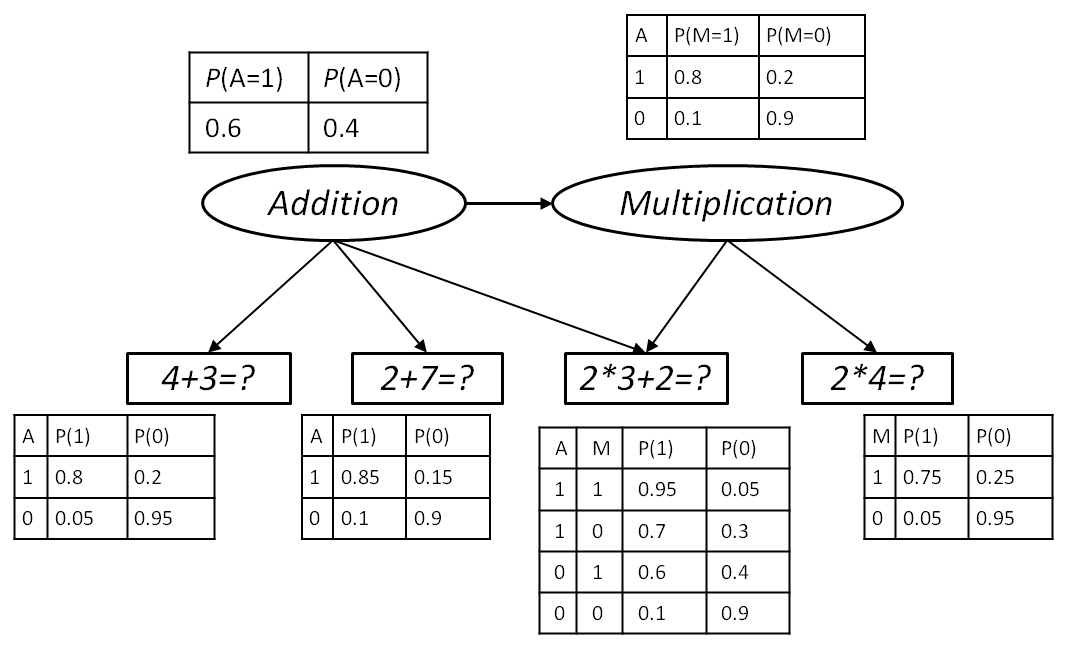
\includegraphics[scale = .48]{figures/studentmodel-as-BN.png}
		\end{center}
	\end{figure}
\end{frame}

\begin{frame}{Prerequisite Discovery as a Machine Learning Problem}
		\begin{itemize}\small
			\item Student performance data (what items a learner answers correctly)
			\item Skill-to-item mapping $Q$-matrix is known
			\item Student's mastery of a skill is unknown $\rightarrow$ latent variables
			\item Learning Bayesian networks with latent variables 
		\end{itemize}

	\begin{figure}[h]
		\begin{center}
			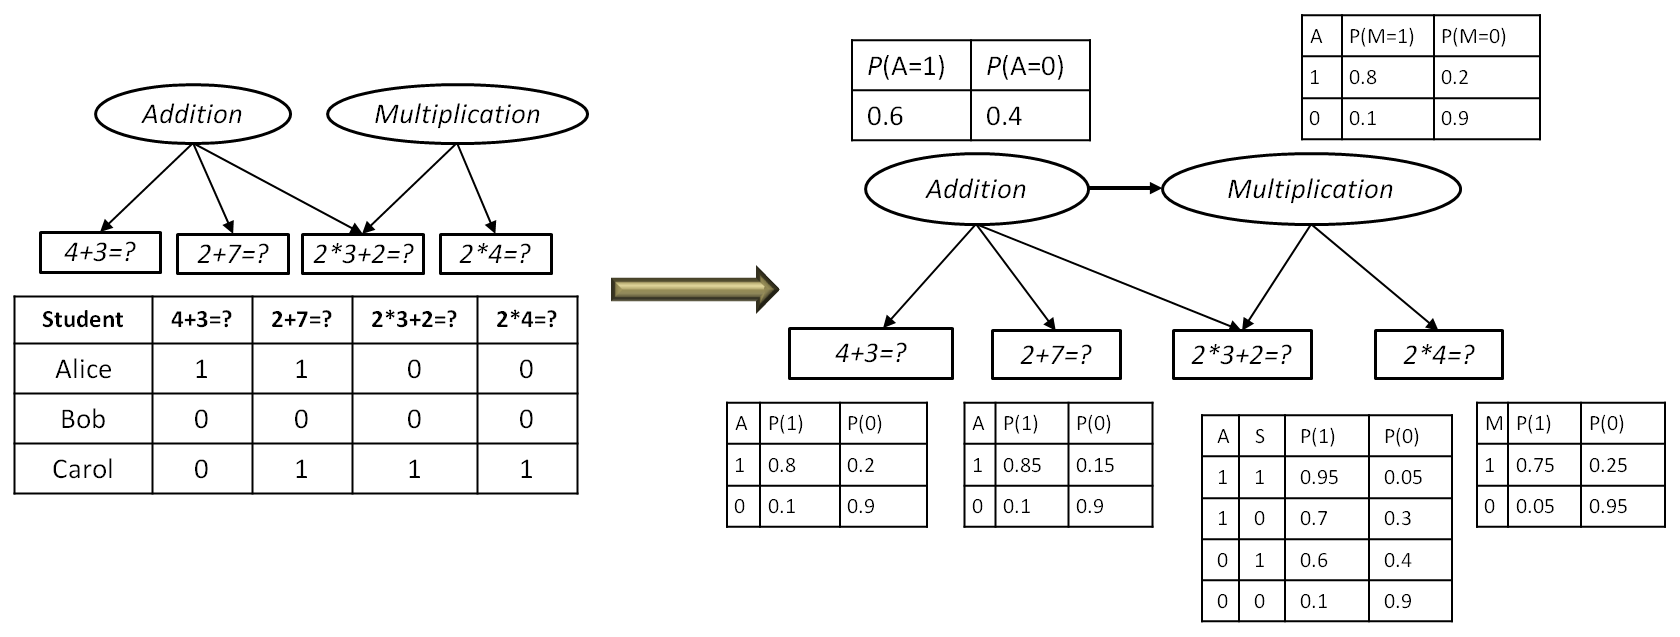
\includegraphics[scale = .4]{figures/prereqdiscovery.png}
		\end{center}
	\end{figure}
\end{frame}

\begin{frame}{Related Prior Work}
	
	\begin{itemize}\small
		\item Brunskill (2010) and Chen et al. (2015)'s work:
		\begin{itemize}
		\item estimated only the pairwise relationships, unable to tell if the relationships are due to indirect   (e.g, $S_3 \rightarrow S_2 \rightarrow S_1$), or direct (e.g, 
		$S_3$\tikz \node(a) {\vphantom{g}};$\rightarrow S_2 \rightarrow$\tikz \node(b) {\vphantom{g}};$S_1$%
		\tikz [overlay] \draw [->]  (a.south) to [bend right=18]  (b.south);) effects.~\\~\\
		\item unclear how to use the output of these relationships for student modeling
		\end{itemize}
		\item K\"{a}ser et al. (2014): manually specified the Bayesian network structure
		\item Scheines et al. (2014): learned the prerequisite graph as a Bayesian network but did not address the issue of Markov equivalence between Bayesian networks.   
	\end{itemize}
	
	\begin{figure}[!ht]\small
		\centering
		\begin{subfigure}[t]{0.3\linewidth}
			\centering
			
\includegraphics[width=0.9\linewidth]{figures/s1s2s3.png}
			\caption{\label{fig:equivnet1}}
		\end{subfigure}
		\begin{subfigure}[t]{0.3\linewidth}
			\centering
			
\includegraphics[width=0.9\linewidth]{figures/s2s1s3.png}
			\caption{\label{fig:equivnet2}}
		\end{subfigure}
		\begin{subfigure}[t]{0.3\linewidth}
			\centering
			
\includegraphics[width=0.9\linewidth]{figures/s3s2s1.png}
			\caption{\label{fig:equivnet3}}			
		\end{subfigure}		
		\caption{Three equivalent BNs representing different prerequisite structures.\label{fig:equivnets} }
	\end{figure}	
\end{frame}

\section{The COMMAND Algorithm}

\begin{frame}{The COMMAND (Combined student Modeling and prerequisite Discovery) Algorithm}
	\begin{figure}[h]
		\begin{center}
			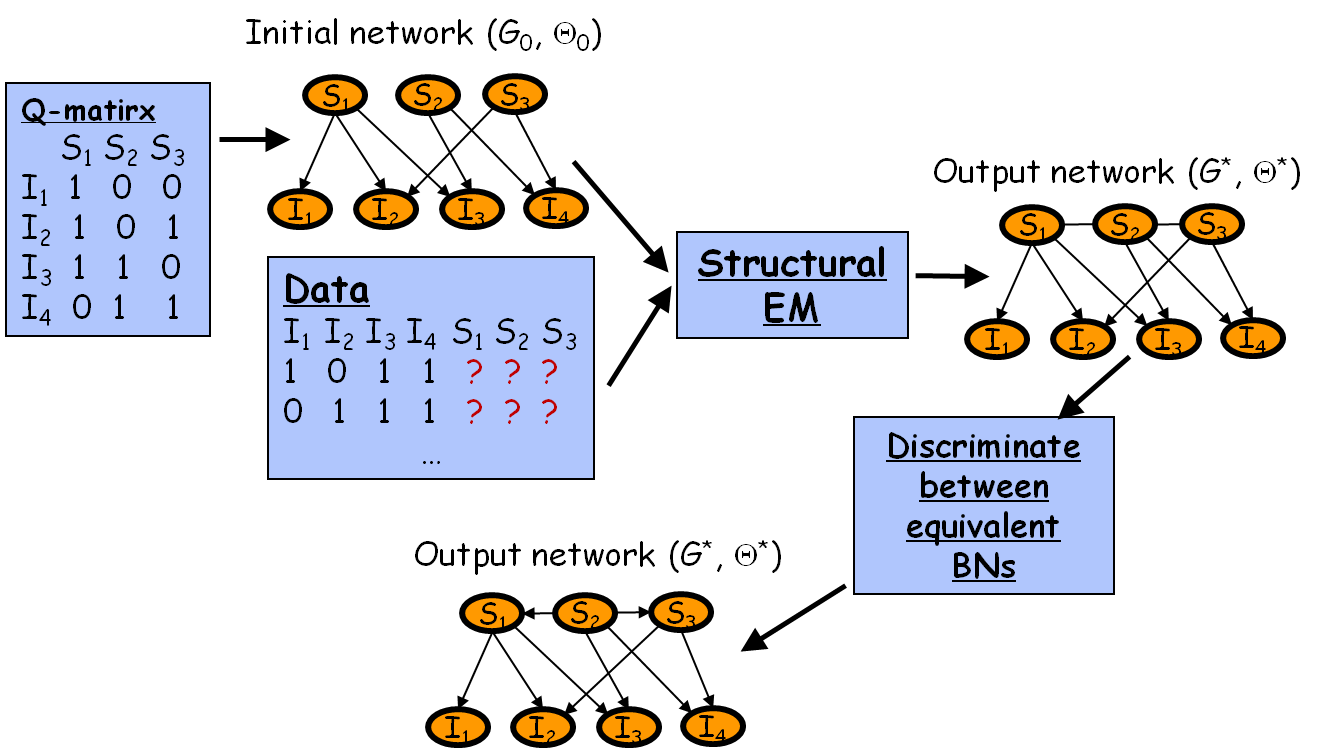
\includegraphics[scale = .5]{figures/command.png}
		\end{center}
	\end{figure}
\end{frame}

\subsection{Structural EM}

\begin{frame}{Learning Bayesian Networks from Data}
\begin{figure}[h]
    \begin{center}
        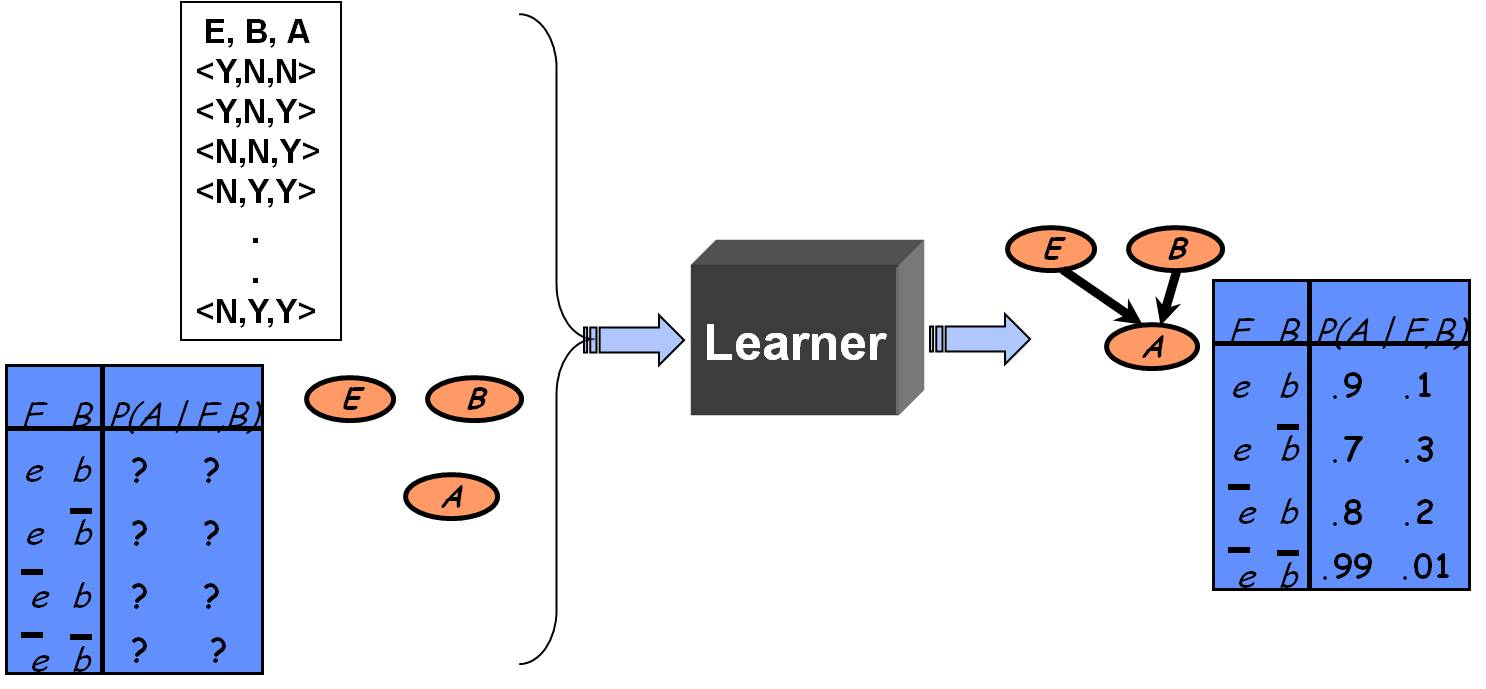
\includegraphics[scale = .4]{figures/learningbn.jpg}
    \end{center}
\end{figure}
Two phases:
\begin{enumerate}
\item Construct the topology (structure) of the networks.
\item Estimate the parameters of the CPDs given the fixed structure.
\end{enumerate}
\end{frame}

\begin{frame}{What Can We Learn?}	
	\begin{enumerate}\small
		\item Assumption: there exists a BN $B$ that \alert{perfectly} represents $P(\mathbf{X})$.
		\item Two BNs are \alert{Markov equivalent} if they represent the same set of CIs.
		\item  Markov equivalent BNs are \alert{statistically indistinguishable} given only observational data.
		%\item Two DAGs are Markov equivalent iff they have the same skeletons and the same $v$-structures.
		\item All Markov equivalent BNs belong to the same \alert{equivalence class} $G^*$ that can be represented by a unique complete partially DAG (CPDAG).
	\end{enumerate}
	\begin{figure}[h]
		\begin{center}
			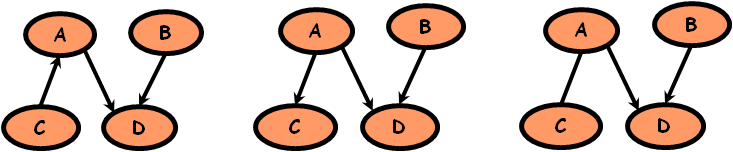
\includegraphics[scale = .6]{figures/markovequiv.png}~\\
			{\small Two Markov equivalent DAGs~~~~~~~~~~CPDAG}
		\end{center}
	\end{figure}			
\end{frame}

\begin{frame}{Score-based Search}
	\begin{itemize}\small
		\item \alert{Score-based search:}
		\begin{itemize}
			\item Solve an optimization problem.
			\item A score to measure the fitness of a DAG to the data: $Score(G:D)=\log P(G,D)$\\
				%The score has closed form solution and can be easily computed from sufficient statistics.
			\item Maximize the score by searching in the space of possible DAGs.% which is $O(n!2^{n(n-1)/2})$.
			\item Local search, e.g., greedy hill climbing, simulated annealing, etc.			
		\end{itemize}
	\end{itemize}
	\begin{figure}[h]
		\begin{center}
			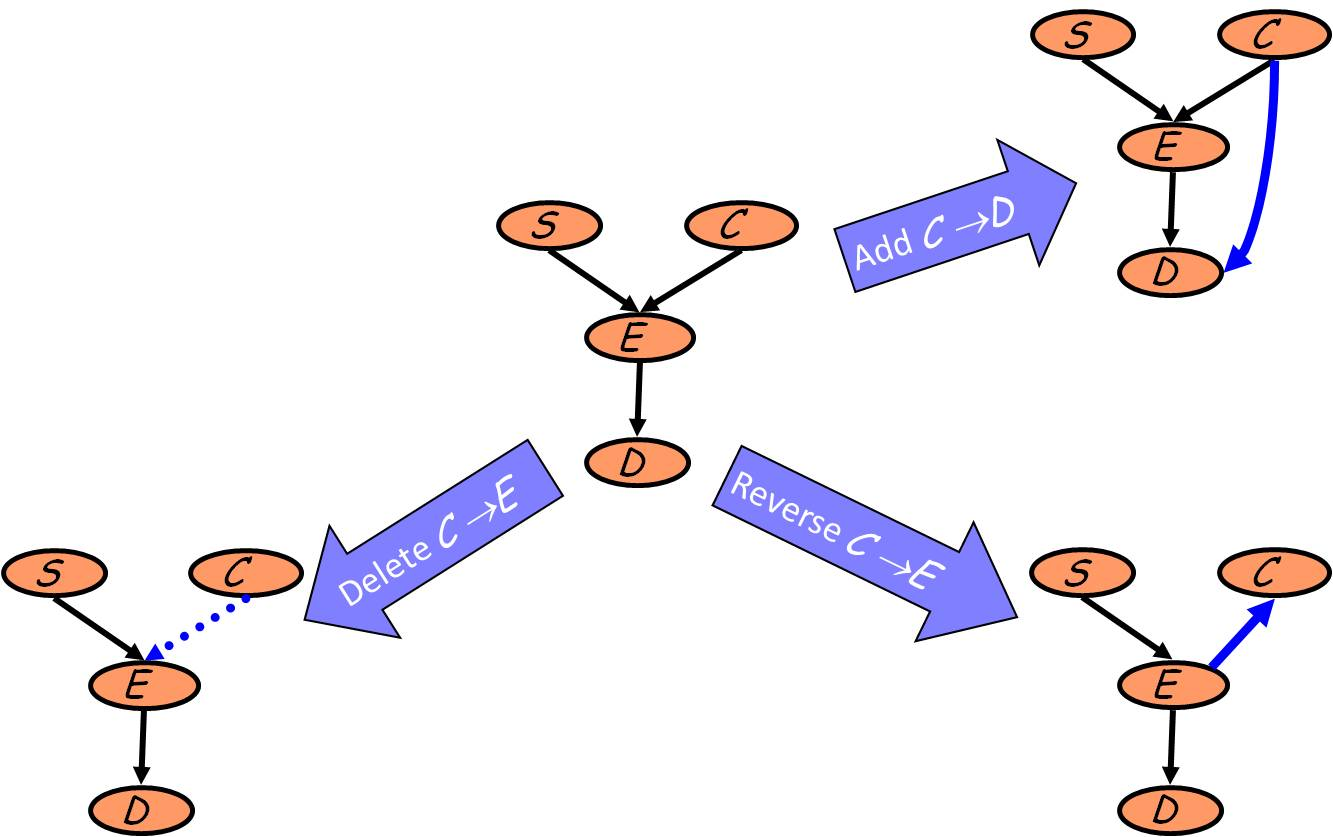
\includegraphics[scale = .3]{figures/structuresearch.jpg}
		\end{center}
	\end{figure}	
\end{frame}

\begin{frame}{What If Some Variables Are Not Observed}

	\begin{itemize}\small
		\item Data contains latent variables or missing values.	
	\end{itemize}		
	\begin{figure}%[h]
		\begin{center}
			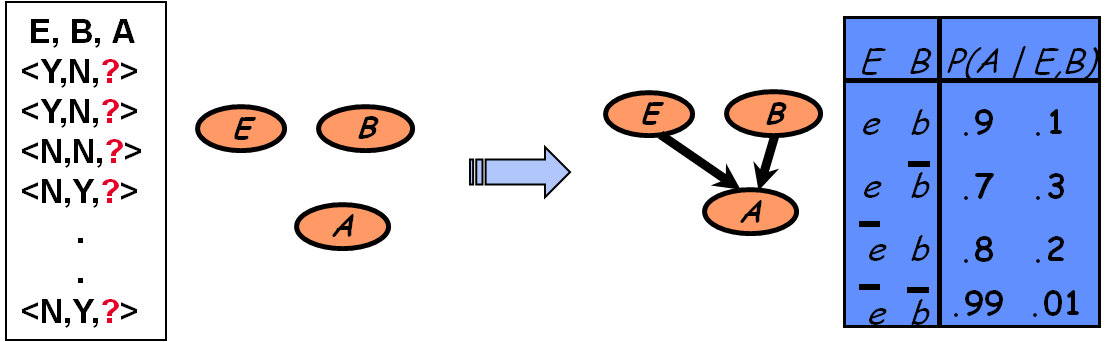
\includegraphics[scale = .5]{figures/bnlatent.png}%\\
			%{\footnotesize We observe $\mathbf{O}= \{E,B\}$, $\mathbf{L}= \{A\}$ is latent.}
		\end{center}
	\end{figure}
	
	\begin{itemize}\small
		\item $Score(G:D)$ has NO closed form solution.
		\item Use iterative algorithm, mostly EM, to estimate $Score(G:D)$.
	\end{itemize}
\end{frame}

\begin{frame}{Traditional EM}	
	\begin{figure}[h]
		\begin{center}
			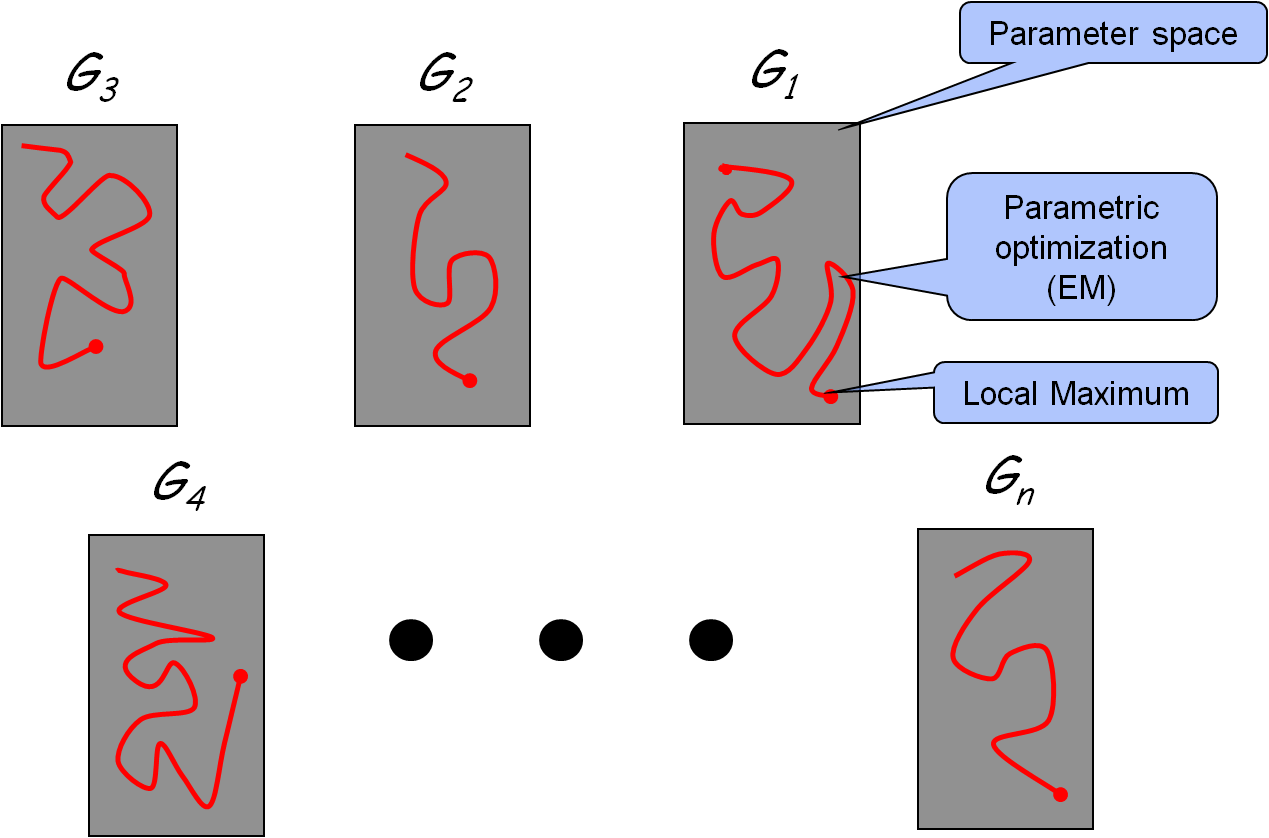
\includegraphics[scale = .35]{figures/traditionalEM.png}%\\
			%{\footnotesize We observe $\mathbf{O}= \{E,B\}$, $\mathbf{L}= \{A\}$ is latent.}
		\end{center}
	\end{figure}
	
	\begin{itemize}\footnotesize
		\item Need run EM for each candidate BN structure.
		\item EM requires BN inference, once for EACH iteration.
		\item EM takes a large (hundreds) number of iterations to converge.
		\item Computationally prohibitive.
	\end{itemize}
\end{frame}

\begin{frame}{Structural Expectation Maximization (Structural EM)}
	\begin{figure}[h]
		\begin{center}
			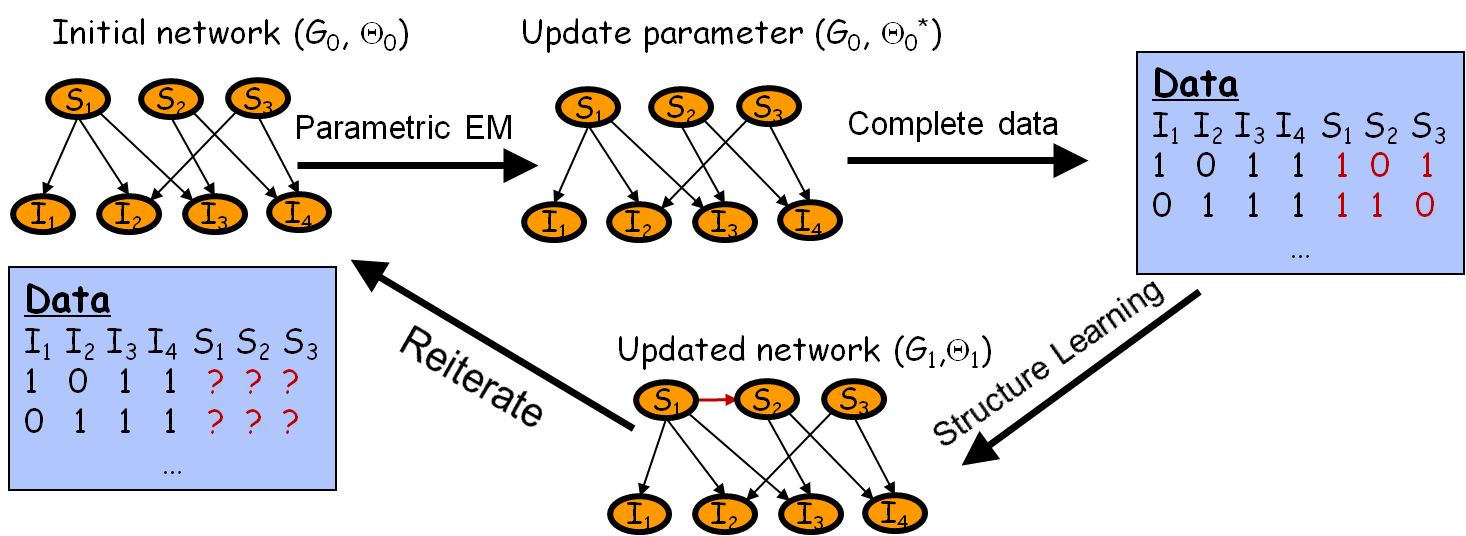
\includegraphics[scale = .48]{figures/sem.png}\\
			{\small (Friedman et al, 1997;1998)}
		\end{center}
	\end{figure}
	Advantage:
	\begin{itemize}\footnotesize
		\item We run EM only on ONE structure, namely the current structure.
	\end{itemize}
\end{frame}

\begin{frame}{Structural EM: Convergence Property}
	\begin{itemize}
		\item $Score(G_t,\theta_t:D)$ increases monotonically with iteration $t$. Hence structural EM converges.\\~\\
		\item $\theta_t$ converges to global or local parametric maxima or saddle points in the parameter space.\\~\\
		\item Not sure the structure converges to what.\\~\\
		\item Empirical results indicates that structural EM finds good structures.
	\end{itemize}
\end{frame}

\subsection{Discriminate Between Equivalent BNs}
	
\begin{frame}{Discriminate Between Equivalent BNs}

	\begin{itemize}
		\item Scoring function used by Structural EM does not discriminate between equivalent Bayesian networks.
	\end{itemize}
			
	\begin{figure}[!ht]\small
		\centering
		\begin{subfigure}[t]{0.3\linewidth}
			\centering
			
\includegraphics[width=0.9\linewidth]{figures/s1s2s3.png}
			\caption{\label{fig:equivnet1_b}}
		\end{subfigure}
		\begin{subfigure}[t]{0.3\linewidth}
			\centering
			
\includegraphics[width=0.9\linewidth]{figures/s2s1s3.png}
			\caption{\label{fig:equivnet2_b}}
		\end{subfigure}
		\begin{subfigure}[t]{0.3\linewidth}
			\centering
			
\includegraphics[width=0.9\linewidth]{figures/s3s2s1.png}
			\caption{\label{fig:equivnet3_b}}			
		\end{subfigure}		
		\caption{Three equivalent BNs \label{fig:equivnets_b} }
	\end{figure}

	\begin{itemize}
		\item We need determine the orientation for every reversible edge.
	\end{itemize}
		
\end{frame}

\begin{frame}{A Heuristic to Orient A Reversible Edge}
	\begin{block}{Assumption}\small
		If $S_1$ is a prerequisite of $S_2$ (i.e., $S_1\rightarrow S_2$), then $S_1=0\Rightarrow S_2=0 $.
		In other words, $P(S_2=\text{0}|S_1=0)=1$.	
	\end{block}

	\begin{block}{Rule}\small
		For every reversible edge, if $ratio=\frac{P(S_2=0|S_1=0)}{P(S_1=0|S_2=0)}\ge 1$, we determine $S_1\rightarrow S_2$; otherwise, we determine $S_1\leftarrow S_2$.	
	\end{block}
	
		\begin{figure}[!ht]\small
			\centering
			\begin{subfigure}[t]{0.32\linewidth}
				\centering
				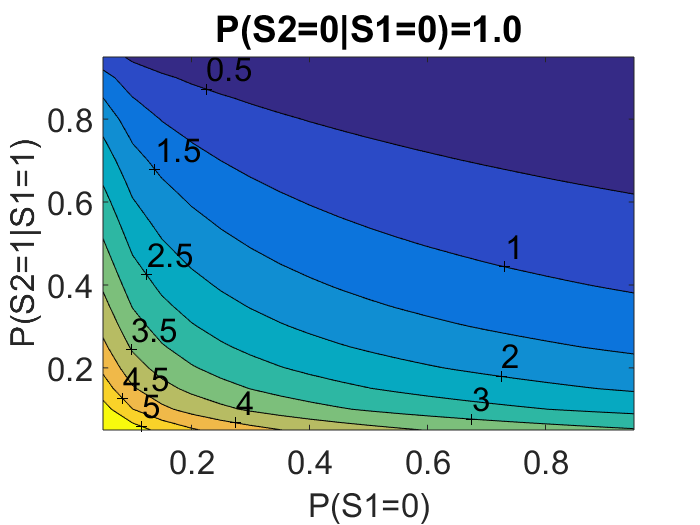
\includegraphics[width=1.0\linewidth]{figures/contour1.png}
				%\caption{\label{fig:contour1}}
			\end{subfigure}
			\begin{subfigure}[t]{0.32\linewidth}
				\centering
				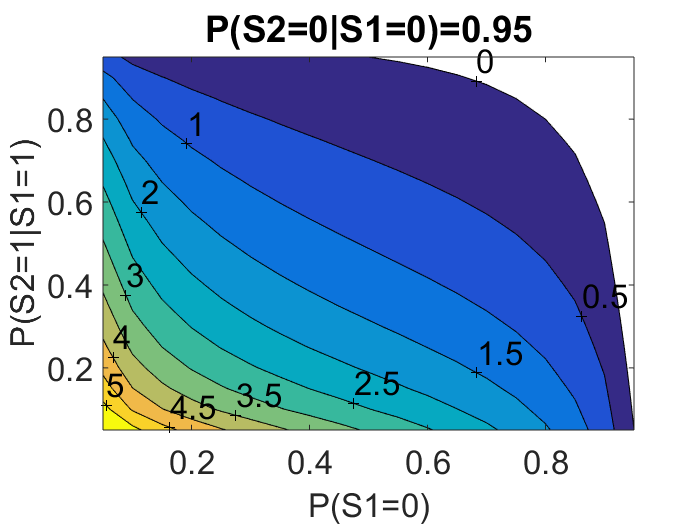
\includegraphics[width=1.0\linewidth]{figures/contour2.png}
				%\caption{\label{fig:contour2}}
			\end{subfigure}
			\begin{subfigure}[t]{0.32\linewidth}
				\centering
				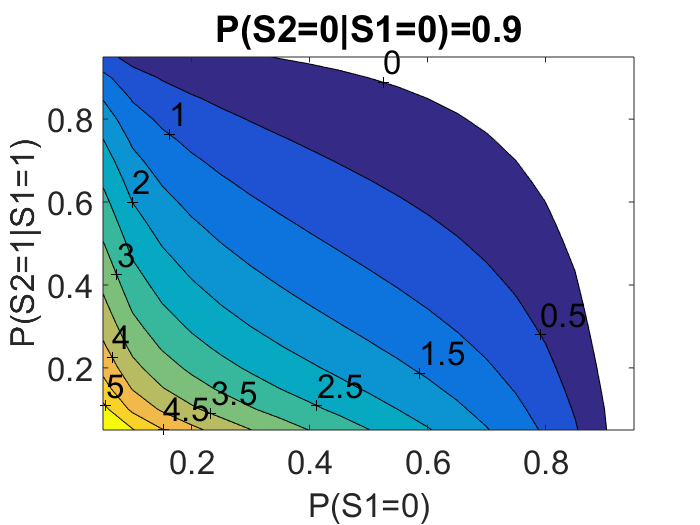
\includegraphics[width=1.0\linewidth]{figures/contour3.png}
				%\caption{\label{fig:contour3}}
			\end{subfigure}						
			\caption{\footnotesize Contour plots of $log(ratio)$ against $P(S_1=0)$ and $P(S_2=1|S_1=1)$ for various values of $P(S_2=0|S_1=0)$.}
		\end{figure}		
\end{frame}

\begin{frame}{An Ad-hoc Strategy to Orient All Reversible Edges}
	
	\begin{enumerate}\small
		\item For each reversible edge $S_i-S_j$, let $ratio^*=ratio$ if $ratio \ge 1$ and $ratio^*=\frac{1}{ratio}$ otherwise. 
		%The larger the $ratio^*$ is, the more confidently when we decide the orientation.
		\item Sort the list of reversible edges by $ratio^*$ in descending order. 
		\item Orient the edges by this ordering using the heuristic rule.
		\item After determine each edge, propagate the constraint to mantain equivalence and acyclicity.
	\end{enumerate}	
	
	\begin{figure}[!ht]\small
		\centering
		\begin{subfigure}[t]{0.24\linewidth}
			\centering
			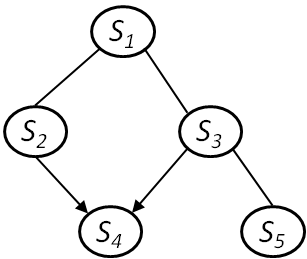
\includegraphics[width=0.95\linewidth]{figures/orient-edges-1.png}
			\caption{\scriptsize 3 reversible edges}
		\end{subfigure}
		\begin{subfigure}[t]{0.24\linewidth}
			\centering
			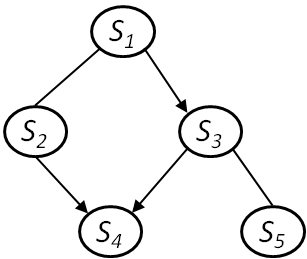
\includegraphics[width=0.95\linewidth]{figures/orient-edges-2.png}
			\caption{\scriptsize Orient $S_1\rightarrow S_3$.}
		\end{subfigure}
		\begin{subfigure}[t]{0.24\linewidth}
			\centering
			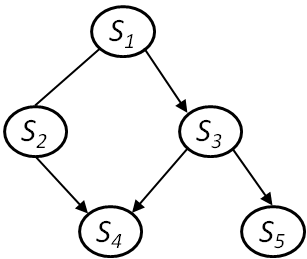
\includegraphics[width=0.95\linewidth]{figures/orient-edges-3.png}
			\caption{\scriptsize Force $S_3\rightarrow S_5$}
		\end{subfigure}	
		\begin{subfigure}[t]{0.24\linewidth}
			\centering
			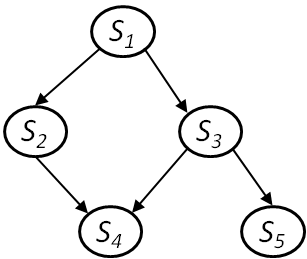
\includegraphics[width=0.95\linewidth]{figures/orient-edges-4.png}
			\caption{\scriptsize Orient $S_1\rightarrow S_2$.}
		\end{subfigure}								
	\end{figure}		
\end{frame}


\section{Evaluation} 
\subsection{Synthetic Data}

\begin{frame}{Evaluation: Synthetic Skill Prerequisite Graph}
	\begin{itemize}\small
		%\item Synthetic Prerequisite Structures of Skills
		\item Each skill node is parent of 6 item variables and each item variable has 1-3 skill nodes as parents.
		\item All of these nodes are modeled using binary random variables. %The latent  nodes represent whether the student achieves mastery of the skill,
		%and the observed nodes indicate if the student answers the item correctly.
		Skill node: mastery or not mastery; item node: correct or incorrect
	\end{itemize}
	\begin{figure}[!ht]\small
		%\begin{center}
		\begin{minipage}[b]{0.3\linewidth}
			\centering
			
\includegraphics[width=0.8\linewidth]{figures/model1.png}\\~\\
			(a) Structure 1~\\~\\~\\
			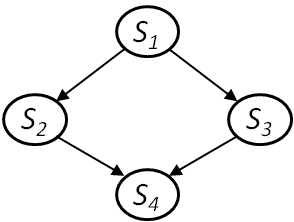
\includegraphics[width=0.7\linewidth]{figures/model2.png}\\~\\
			(b) Structure 2
		\end{minipage}
		\quad
		\begin{minipage}[b]{0.3\linewidth}
			\centering
			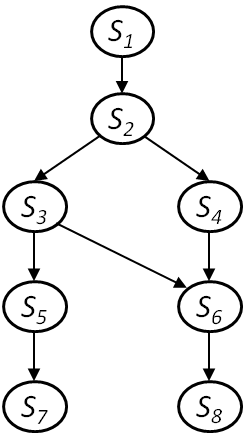
\includegraphics[width=0.6\linewidth]{figures/model3.png}\\~\\
			(c) Structure 3
		\end{minipage}	
		\caption{Item nodes are omitted.}
		\label{fig:syn-nets}
		%\vspace{-1em}
		%\end{center} 
	\end{figure}
\end{frame}

\begin{frame}{Evaluation With Synthetic Data}
	We designed experiments to specifically answer the following four questions:
	\begin{enumerate}\small
		\item How does the type of items affect COMMAND's ability to recover the prerequisite structure?
		\alert{Single-skilled items v.s. multi-skilled items}. 
		\item How well does COMMAND perform when there is noise in the data?
		\alert{Data contains noise due to the presence of unaccounted latent variables}.
		\item How well does COMMAND perform when the student performance data have \alert{missing values}?
		\item How is COMMAND compared with other prerequisite discovery methods?
		Compare COMMAND to the Probabilistic Association Rules Mining (PARM) method (Chen et al., 2015).
	\end{enumerate}
\end{frame}

\begin{frame}{Evaluation Metrics}
	\begin{table}%[ht]
		\centering
		\caption{Formulas for measuring adjacency rate (AR)}
		%\label{my-label}
		\begin{tabular}{@{}ll@{}}
			%\toprule
			\hline
			Metric & Formula \\ %\midrule
			\hline
			True positive    (\emph{TPAR}) & $\frac{ \text{\# of correct adjacencies in learned model} } { \text{ \# of adjacencies in true model} }$  \\
			True discovery (\emph{TDAR}) &  $\frac{ \text{\# of correct adjacencies in learned model} } { \text{ \# of adjacencies in learned model} }$ \\
			$F_1$-\textit{AR} &  $\frac{2\cdot \text{\emph{TPAR}} \cdot \text{\emph{TDAR}}} {\text{\emph{TPAR}}+\text{\emph{TDAR}}}$  \\
			\hline
		\end{tabular}
	\end{table}
	\vspace{-1em}
	\begin{table}[ht]
		\centering
		\caption{Formulas for measuring orientation rate (OR)}
		%\label{my-label}
		\begin{tabular}{@{}ll@{}}
			%\toprule
			\hline
			Metric & Formula \\ %\midrule
			\hline
			True positive  (\emph{TPOR}) & $\frac{ \text{\# of correctly directed edges in learned model} } {\text{ \# of directed edges in true model}}$  \\
			True discovery   (\emph{TDOR})& $\frac{ \text{\# of correctly directed edges in learned model } }{\text{ \# of directed edges in learned model}} $\\
			$F_1$-\textit{OR} &  $\frac{  2\cdot \text{\emph{TPOR}} \cdot \text{\emph{TDOR}} }{\text{\emph{TPOR}}+\text{\emph{TDOR}}}$ \\
			%\bottomrule
			\hline
		\end{tabular}
	\end{table}
\end{frame}


\begin{frame}{Synthetic Data: Single-skilled vs Multi-skilled Items}
	\begin{figure}[ht]
		\begin{center}
			\begin{tabular}{>{\centering}m{1.5in} >{\centering\arraybackslash}m{1.5in}}
				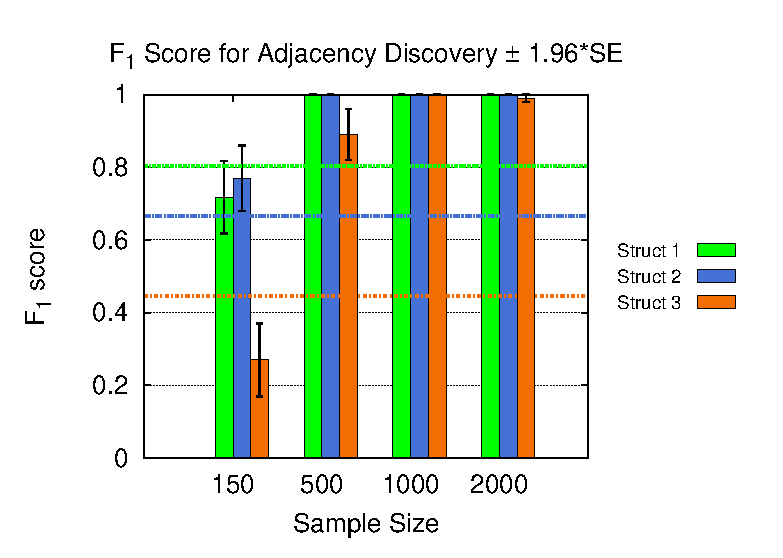
\includegraphics[width=1.1\linewidth]{figures/F1A_single.eps} &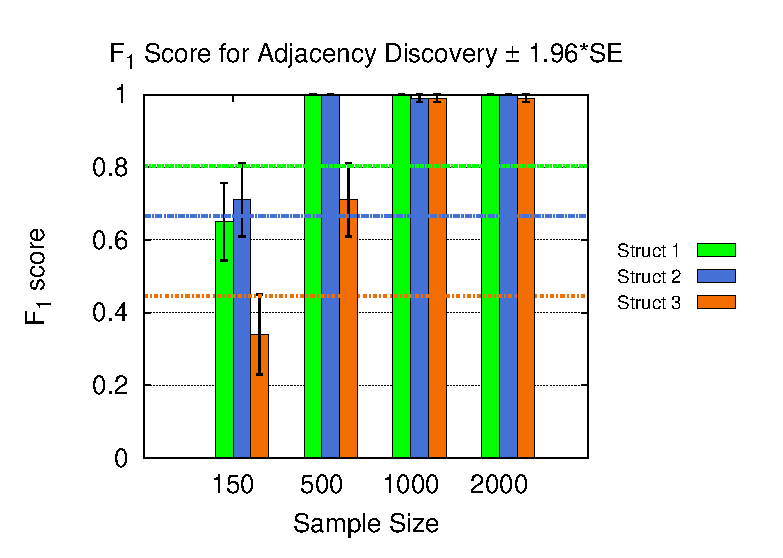
\includegraphics[width=1.1\linewidth]{figures/F1A_multi.eps}\\
				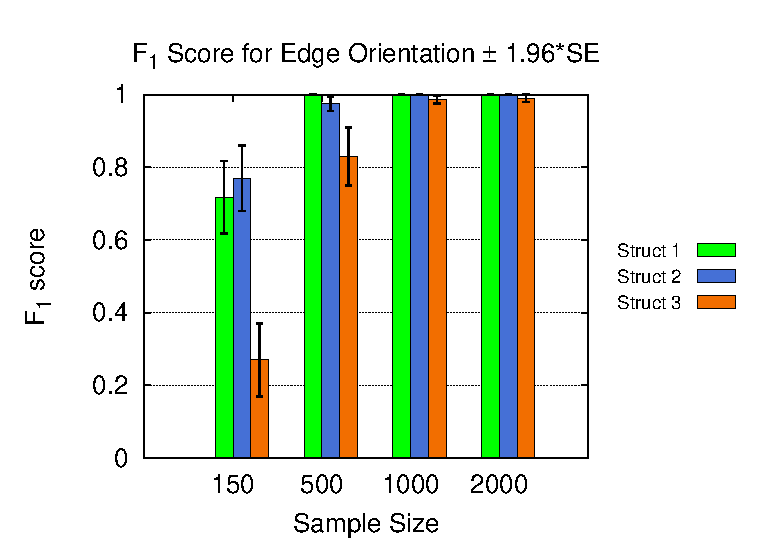
\includegraphics[width=1.1\linewidth]{figures/F1O_single.eps} &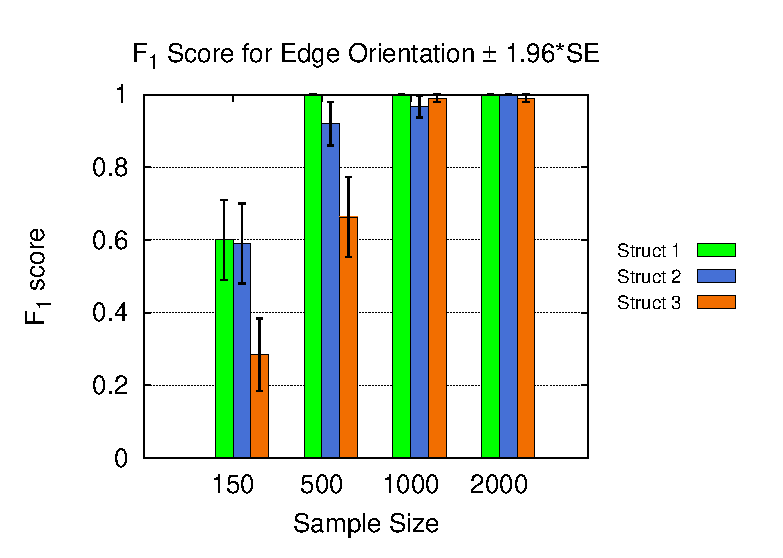
\includegraphics[width=1.1\linewidth]{figures/F1O_multi.eps}\\
				{\small Single Skill}& {\small Multiple Skill}
			\end{tabular}
		\end{center}
		\caption{\footnotesize Comparison of $F_1$ scores for adjacency discovery (top row) and for edge orientation (bottom row). 
			%Horizontal lines are baseline scores for fully-connected (complete) networks.
			%The error bars show the $95\%$ confidence intervals, i.e., $\pm 1.96*$\texttt{SE}.
			} 
		\label{fig:f1-single-multi}
	\end{figure} 
\end{frame}

\begin{frame}{Evaluation of COMMAND With Noisy Data}
	\begin{itemize}\small
		\item Noise may occur due to the presence of latent variables that are not explicitly modeled, e.g., student ability.
		\item Students' performance depends not only on whether they have mastered the skills, but also on their individual ability
		\item Synthesized BN models including an extra variable \emph{StudentAbility} with 3 possible states (low/med/high). 
	\end{itemize}
	\begin{figure}[h]
		\begin{center}
			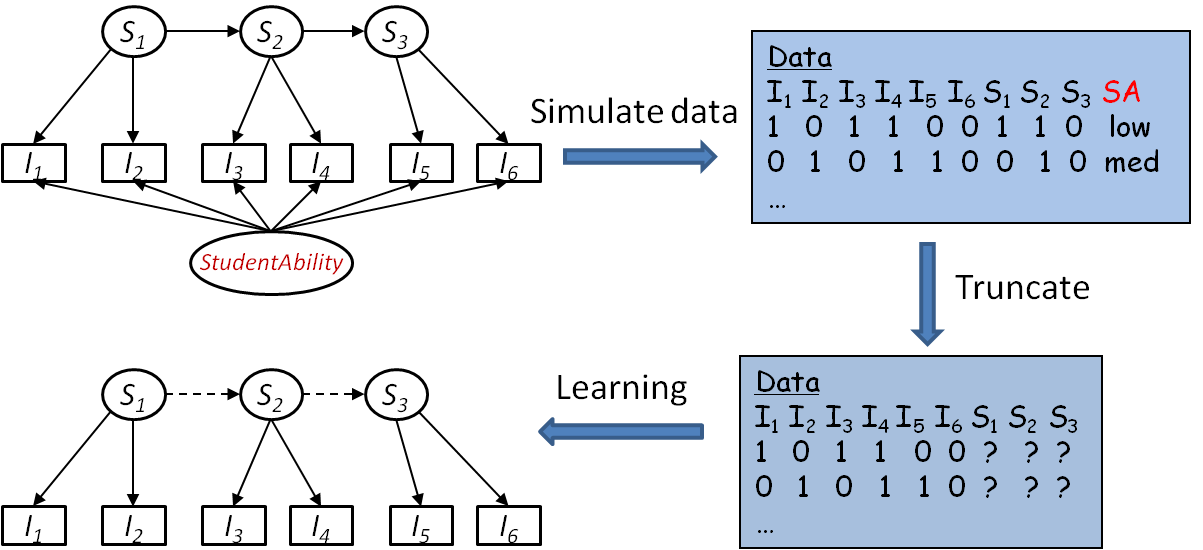
\includegraphics[scale = .45]{figures/studentability.png}
		\end{center}
	\end{figure}	
\end{frame}

\begin{frame}{Results: Sensitivity to Noise}
			\begin{figure}[!ht]
				\begin{center}
					\centering
					\begin{tabular}{>{\centering}m{1.5in} >{\centering\arraybackslash}m{1.5in}}
						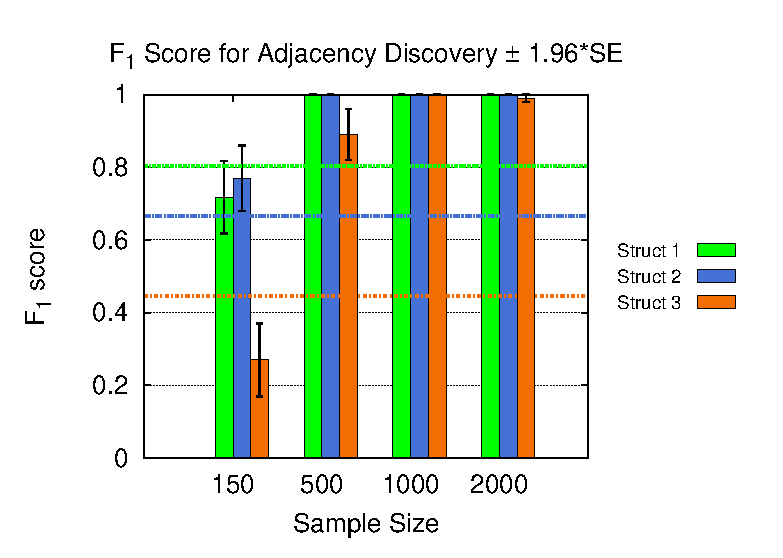
\includegraphics[width=1.1\linewidth]{figures/F1A_single.eps} &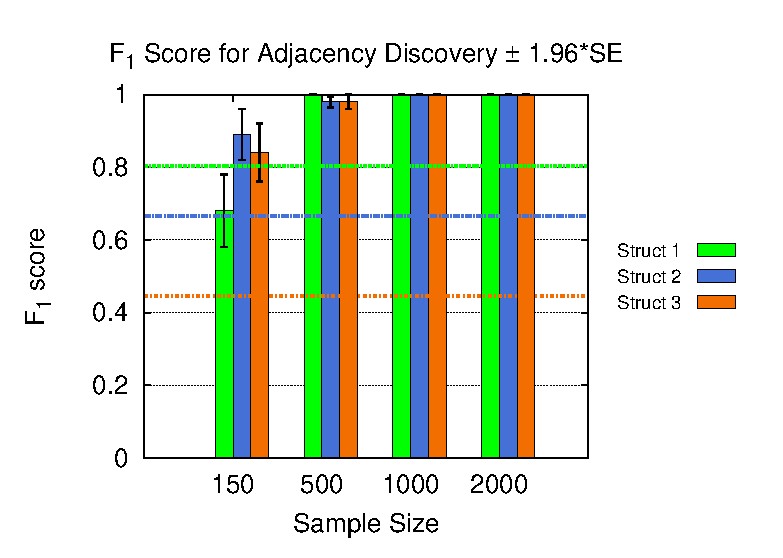
\includegraphics[width=1.1\linewidth]{figures/F1A_single_noisy.eps}\\
						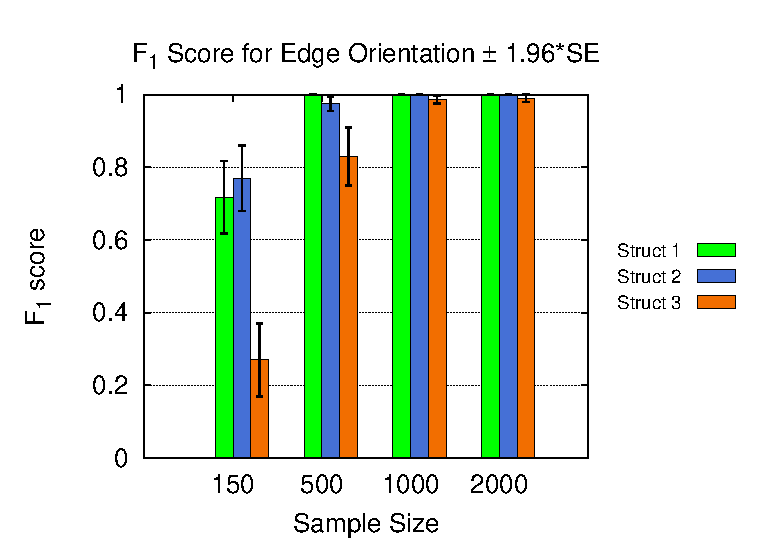
\includegraphics[width=1.1\linewidth]{figures/F1O_single.eps} &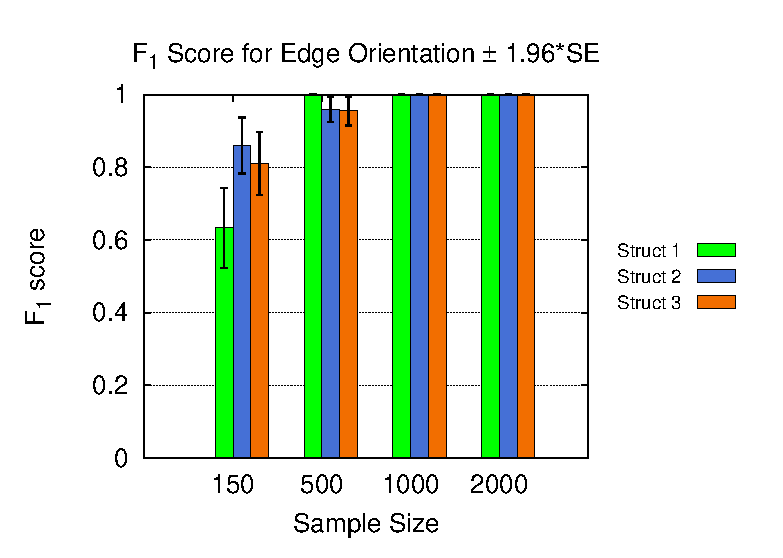
\includegraphics[width=1.1\linewidth]{figures/F1O_single_noisy.eps}\\
						No Noise & Noisy
					\end{tabular}
				\end{center}
				%\vspace{-1em}
				\caption{\footnotesize Results of adding systematic noise. Comparison of $F_1$ scores for adjacency discovery (top row) and for edge orientation (bottom row).}
				\label{fig:f1-noisy} 
			\end{figure}
\end{frame}

\begin{frame}{Data Containing Missing Values}
	\begin{itemize}\small
		\item Real-world datasets collected from students often have missing values, for example, when  learners  do not answer  all items.
		\item COMMAND can be applied on data containing missing values. 
	\end{itemize}
\begin{table}[htb]\small
	\centering
	\caption{Example student performance matrix containing missing values.}
	\begin{tabular}{@{}lllll@{}}
		\hline
		User  & Item 1 & Item 2 & Item 3 & Item $p$ \\ \hline
		Alice & 0      & ?      &        & 0        \\
		Bob   & ?      & 1      & ...    & 1        \\
		Carol & 0      & 0      &        & ?        \\
		\multicolumn{5}{c}{...}                     \\ \hline
	\end{tabular}
\end{table}	
\end{frame}

\begin{frame}{Data Containing Missing Values}
	\begin{itemize}\small
		\item We generated data sets of with 1000 observations with varying fraction of randomly missing values ($10\%$, $20\%$, $30\%$, $40\%$, $50\%$). 
	\end{itemize}
		\begin{figure}[ht]
			\begin{center}
				\centering
				\begin{tabular}{>{\centering}m{2.0in} >{\centering\arraybackslash}m{2.0in}}
					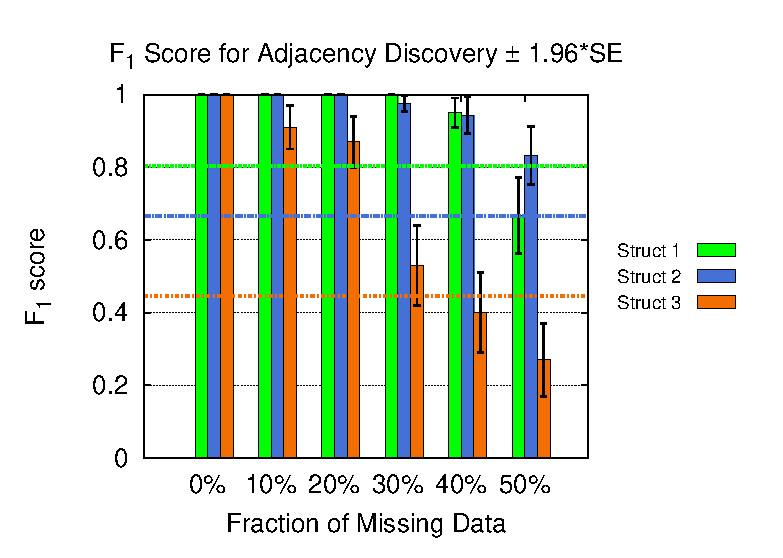
\includegraphics[width=1.1\linewidth]{figures/F1A_single_missing.eps} &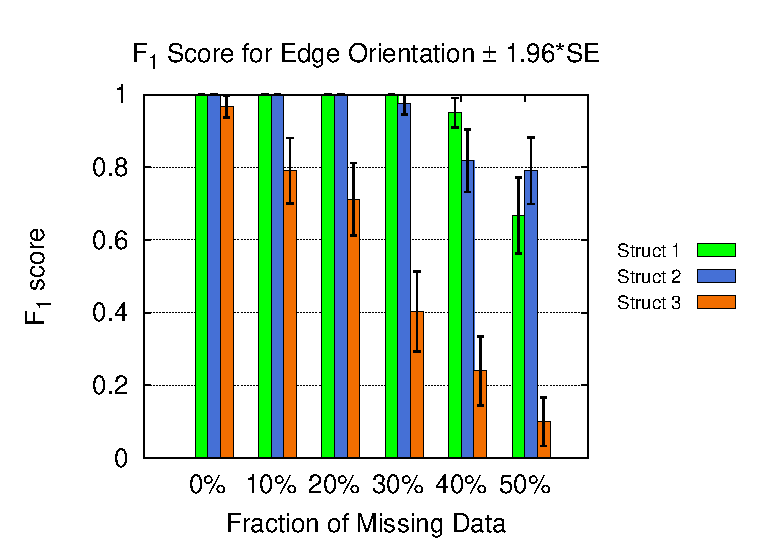
\includegraphics[width=1.1\linewidth]{figures/F1O_single_missing.eps}\\
				\end{tabular}
			\end{center}
			%\vspace{-1em}
			\caption{\footnotesize Results of learning with missing data. Comparison of $F_1$ scores for adjacency discovery (left) and for edge orientation (right). }
			\label{fig:f1-missing} 
		\end{figure}	
\end{frame}

\begin{frame}{Comparison With Prior Work}
	\begin{itemize}\small
		\item Probabilistic Association Rules Mining (PARM) (Chen et al., 2015): a recent algorithm for discovering the \alert{pairwise} prerequisite relationships.
		\item A prerequisite relationship $S_1\rightarrow S_2$ is considered to exist if
		$P(S_1=1,S_2=1) \ge minsup \wedge P(S_1=1|S_2=1)\ge minconf) \ge minprob$ and $P(P(S_1=0,S_2=0) \ge minsup \wedge P(S_2=0|S_1=0)\ge minconf) \ge minprob$. 
		\item Need expert to specify the thresholds $minsup$, $minconf$ and $minprob$.
	\end{itemize}
%			\begin{figure}[ht]
%				\begin{center}
%					\centering
%					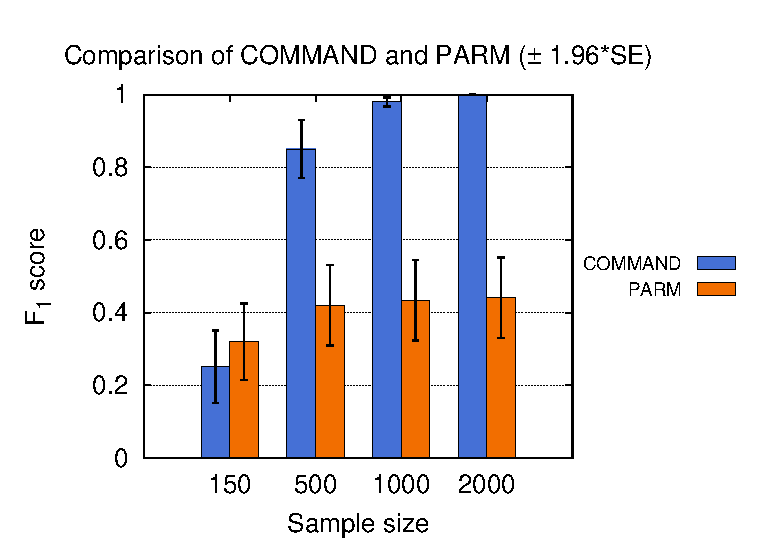
\includegraphics[width=0.45\linewidth]{figures/F1_parm.eps}
%				\end{center}
%				%\vspace{-1em}
%				\caption{\footnotesize Comparison of COMMAND and PARM for discovering prerequisite relationships in Structure 3. The cutoff values used for PARM experiments are: $ minsup=0.125$, $minconf=0.76$, $minprob=0.9$.
%				}
%				\label{fig:f1-parm}
%				%\vspace{-1em} 
%			\end{figure}
	\begin{figure}[!ht]\small
		\centering
		\begin{subfigure}[t]{0.49\linewidth}
			\centering
			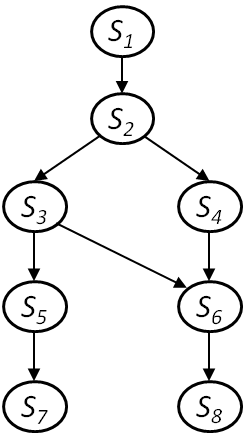
\includegraphics[width=0.3\linewidth]{figures/model3.png}
			\caption{\footnotesize 21 pairwise relationships}
		\end{subfigure}
		\begin{subfigure}[t]{0.49\linewidth}
			\centering
			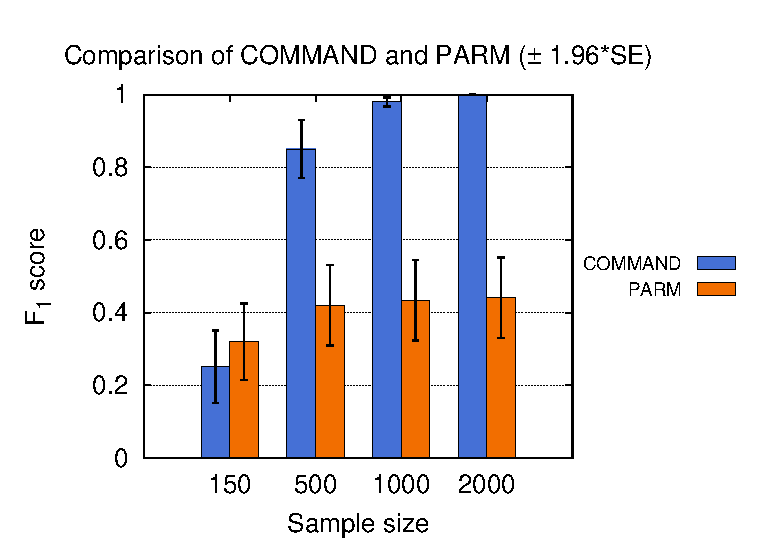
\includegraphics[width=0.8\linewidth]{figures/F1_parm.eps}
			\caption{\footnotesize $ minsup=0.125$, $minconf=0.76$, $minprob=0.9$ are used for PARM.}
		\end{subfigure}							
	\end{figure}		
\end{frame}			

\subsection{Real-World Data}

\begin{frame}{English Data Set}
	\begin{itemize}\small 
		\item The Examination for the Certification of Proficiency in English (ECPE) dataset (Templin and Bradshaw, 2014):
		\begin{itemize}
		\item 2922 examines in their understanding of English language grammar .
		\item student performance in 28 items on 3 skills \\
		(\textbf{$S_1$: morphosyntactic rules, $S_2$: cohesive rules, and $S_3$:lexical rules}). 
		\item Each item requires either one or two of the three skills.	
		\end{itemize}	
\end{itemize}

				\begin{figure}[!th]
					\begin{center}
						\centering
						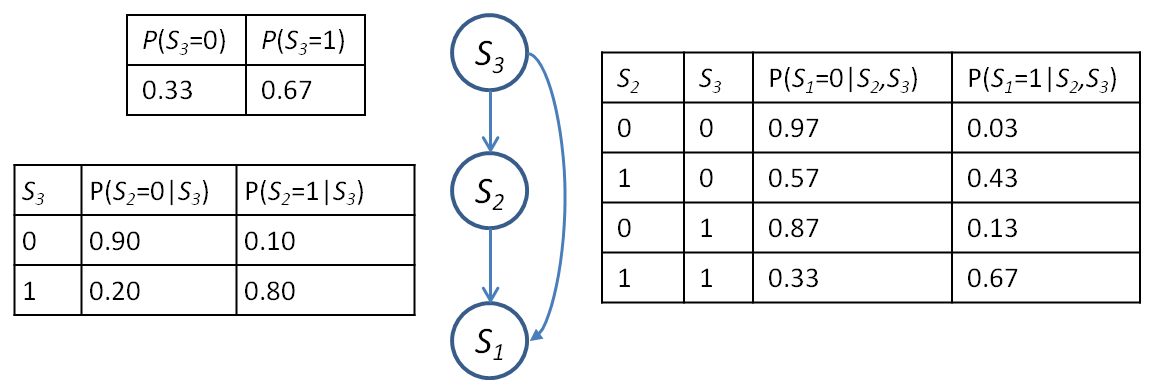
\includegraphics[width=0.9\linewidth]{figures/ecpe_results.png}
					\end{center}
					%\vspace{-1em}
					\caption{%$S_1$: Morphosyntactic rules; $S_2$: Cohesive rules; $S_3$: Lexical rules. 
						\footnotesize The estimated DAG and CPTs of the ECPE data set.}
					\label{fig:ecpe-result} 
					%\vspace{-0.5em}
				\end{figure}
\end{frame}

\begin{frame}{Math Data Set}
	\begin{itemize}\small 
		\item Collected from a commercial non-adaptive tutoring system.
		\item The textbook items are classified in chapters, sections, and objectives.
		\item Define skills as book sections and use a $Q$-matrix that assigns each exercise to a skill solely as the book section in which the item appears.
	\end{itemize}

				\begin{figure}[!th]
						\centering
						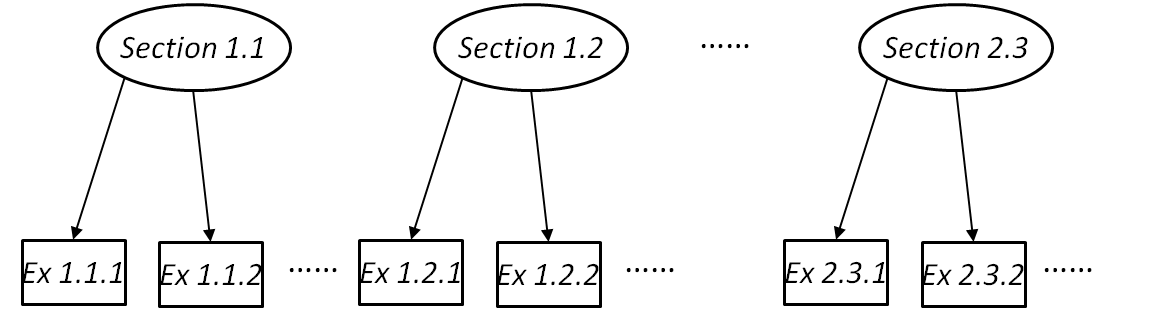
\includegraphics[width=0.9\linewidth]{figures/mathdataset.png}
				\end{figure}	
	
\end{frame}

\begin{frame}{Math Data Set: Constructed Prerequisite Graph}
	\begin{figure}[!ht]
		\centering
		\begin{subfigure}[b]{0.49\linewidth}
			\centering
			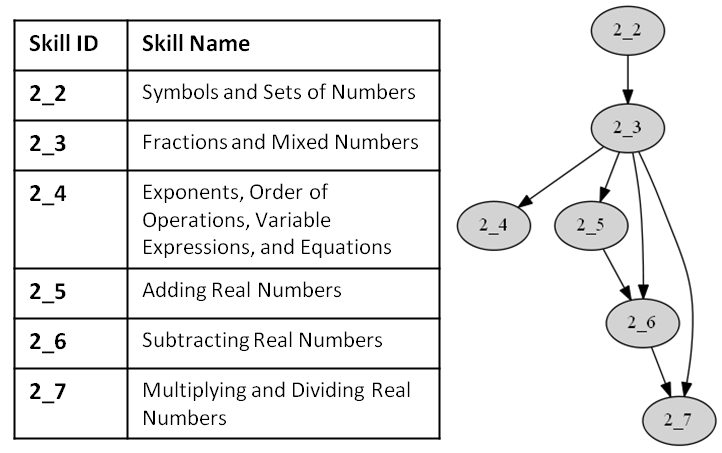
\includegraphics[width=0.95\linewidth]{figures/hed_chap2_structure_prob2.png}
			\caption{\texttt{Math-chap2}.}
			\label{fig:hed_chap2_structure}
		\end{subfigure}
		\begin{subfigure}[b]{0.49\linewidth}
			\centering
			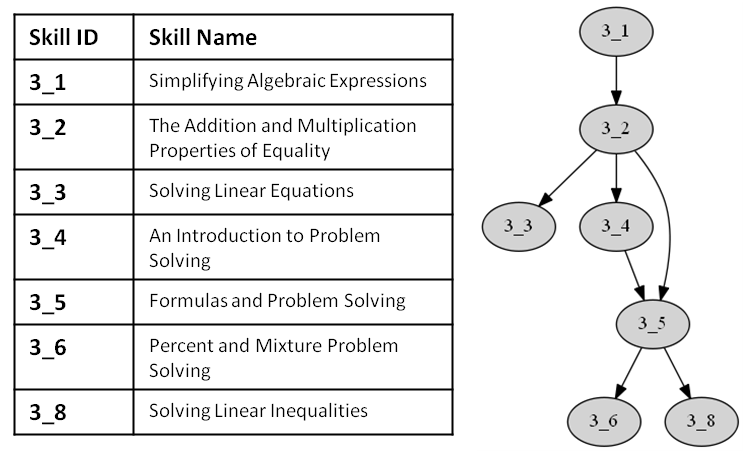
\includegraphics[width=0.95\linewidth]{figures/hed_chap3_structure_prob2.png}
			\caption{\texttt{Math-chap3}.}
			\label{fig:hed_chap3_structure}
		\end{subfigure}%
		\caption{Prerequisite structures constructed by COMMAND for \texttt{Math} data sets.}
		\label{fig:hed-structures}
		%\vspace{-1em} 
	\end{figure}		
	
\end{frame}


\begin{frame}{Predictive Performance}
	We evaluate the accuracy of the predicted student performance on an item, when we observe the student response on the other items. We compare our model with five baseline models:
\begin{itemize}\small
		\item  A \emph{majority} classifier which always classifies an instance to the majority class.
		%For example, if majority of the students get an item wrong, other students would likely get it wrong.
		\item  A Bayesian network model in which the skill variables are \emph{disconnected}. 
		%This corresponds to using the $Q$-matrix  Bayesian network of Figure~\ref{fig:qmatrix}.
		%This model assumes that the skill variables are marginally independent of each other. Most existing knowledge tracing approaches make this assumption.
		\item A Bayesian network model in which the skill variables are connected in a \emph{chain} structure, i.e., 2-2$\rightarrow$2-3$\rightarrow$2-4$\rightarrow\dots$
		%This assumes that a section (skill) only depends on the previous section.
		\item A Bayesian network model constructed using the pairwise relationships output from \emph{PARM}. 
		%That is, we create an edge $S_i\rightarrow S_j$ if PARM says $S_i$ is the prerequisite of $S_j$.
		\item A \emph{fully connected} Bayesian network where skill variables are fully connected with each other.
		%This model assumes no conditional independence between skill variables and can encode any joint distribution over the skill variables.
		%However, it has exponential number of free parameters and thus can easily overfit the data.
\end{itemize}
	\begin{figure}[h]
		\begin{center}\small
			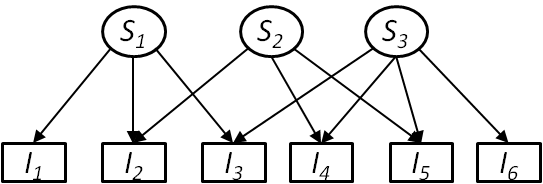
\includegraphics[scale = .4]{figures/disconnected.png}~~
			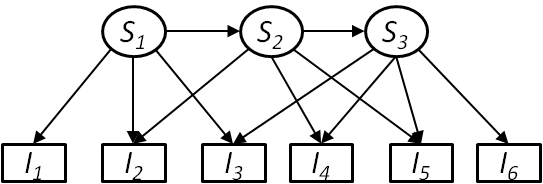
\includegraphics[scale = .4]{figures/chain.png}~~
			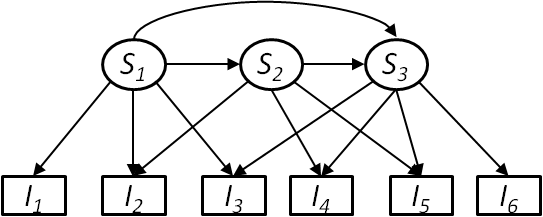
\includegraphics[scale = .4]{figures/fullconnected.png}~\\
			Disconnected~~~~~~~~~~~~~~~~~~~~~Chain~~~~~~~~~~~~~~~~~~Fully connected
		\end{center}
	\end{figure}
\end{frame}

\begin{frame}{Predictive Performance}
	\begin{figure}[!ht]
		\centering
		\begin{subfigure}[b]{0.48\linewidth}
			\centering
			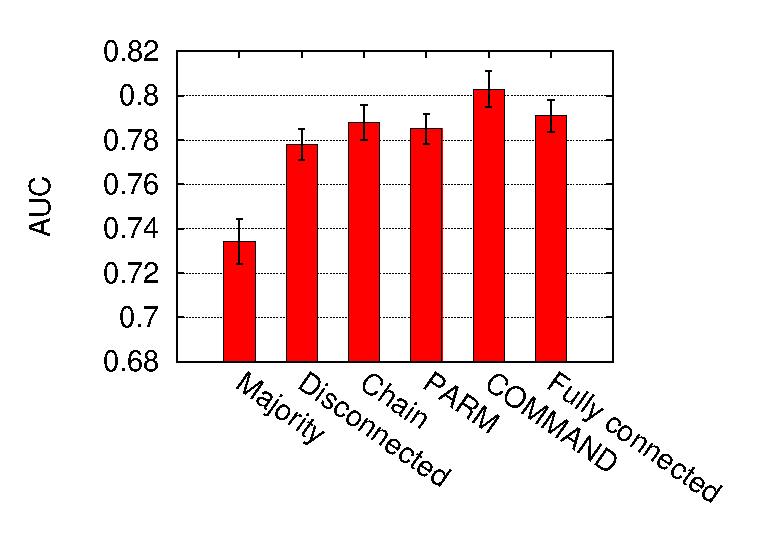
\includegraphics[width=1.1\linewidth]{figures/hed_chap2_30_auc.eps}
			%\vspace{-1em}
			\caption{\texttt{Math-chap2} AUC results. }
			\label{fig:auc-chap2}
		\end{subfigure}
		\begin{subfigure}[b]{0.48\linewidth}
			\centering
			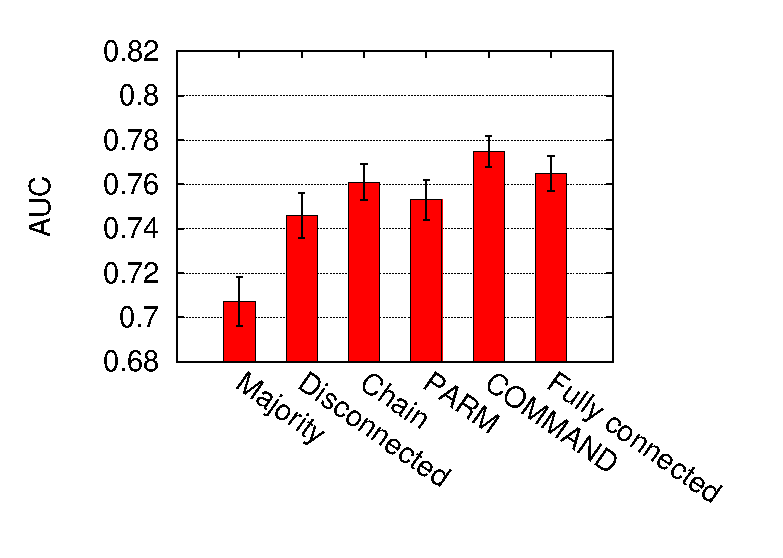
\includegraphics[width=1.1\linewidth]{figures/hed_chap3_33_auc.eps}
			%\vspace{-1em}
			\caption{\texttt{Math-chap3} AUC results.}
			\label{fig:auc-chap3}
		\end{subfigure}%
		%\vspace{-0.5em}
		\caption{\footnotesize Ten fold cross-validation results of evaluating the predictions of student performance.} %\hl{why does the y-axis start at 0.68? consider 0.5}
		\label{fig:aucs}
		%\vspace{-1em}
	\end{figure} 
\end{frame}

\section{Conclusion}
\begin{frame}{Conclusion}
\begin{itemize}
	\item Main contribution: a novel algorithm that simultaneously infers \alert{a prerequisite graph} and \alert{a student model} from data with less human intervention.
	\begin{itemize}
		\item Optimizes the full structure of skills that captures the \alert{conditional independence} between skills. Our experiments suggests that this results in better accuracy.
		\item Easier to use because it does not require  manual tuning of  parameters.
		\item Tolerates missing values in data.
	\end{itemize}
	\item We develop a methodology to evaluate  prerequisite structures on real student data.
	\item Learning a prerequisite graph is not merely discovering a Bayesian network--- 
	\alert{equivalent Bayesian network structures} in fact represent different prerequisite structures.
	We proposed a theoretically motivated method to discriminate between equivalent Bayesian networks.
\end{itemize}
\end{frame}


%\section*{}
%\begin{frame}
%	\frametitle{Questions?}
%	%\begin{block}\large{} \centering Any questions?\end{block}
%	\begin{figure}[h]
%		\begin{center}
%			\includegraphics[scale = .6]{image/50questions.jpg}
%		\end{center}
%	\end{figure}
%\end{frame}

\end{document}

